\documentclass[t,table,usenames,dvipsnames]{beamer}

\usetheme{CambridgeUS}
\usecolortheme{beaver}
\setbeamertemplate{navigation symbols}{}

\usepackage[utf8]{inputenc}
\usepackage[croatian]{babel}

\usepackage{datetime}
\renewcommand{\dateseparator}{.}
\newcommand{\todayiso}{\twodigit\day \dateseparator \twodigit\month \dateseparator \the \year}
\date{\todayiso}

\usepackage{listing}
\usepackage{graphicx}
\usepackage{subcaption}
\usepackage{multirow}
\usepackage{color}
\definecolor{LightGray}{gray}{0.9}
\captionsetup{compatibility=false}

\title[NKOSL]{Napredno korištenje operacijskog sustava Linux}
\author[Dominik Barbarić]{Dominik Barbarić\\{\small Nositelj: doc.dr.sc. Stjepan Groš}}
\subtitle{6. Grafika i zvuk}
\institute[FER]{Sveučilište u Zagrebu\\Fakultet elektrotehnike i računarstva}

\begin{document}

{
	\setbeamertemplate{footline}{}
	\begin{frame}
		\maketitle
	\end{frame}
}

\begin{frame}
	\frametitle{Sadržaj}
	\tableofcontents
\end{frame}



\section{Grafički sustav}


\begin{frame}
	\frametitle{X11}
	\begin{itemize}
		\item Sustav koji povezuje aplikacije (klijente) s grafičkim serverom
		\item X sustav razvijen na MIT 1984. godine
		\item U verziji X11 od 1987. godine. Male nadogradnje održavaju korak s razvojem grafičkih sustava
		\item[]
		\item \emph{Xorg server}
	\end{itemize}
\end{frame}


\begin{frame}
	\frametitle{X11}
	\begin{itemize}
		\item Aplikacije koriste X kroz framework za crtanje grafičkih elemenata
		\item Uređivanje prikaza svih aplikacija obavlja \emph{window manager}
	\end{itemize}
	
	\begin{figure}[h]
		\begin{minipage}{0.25\textwidth}
			\centering
			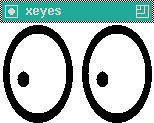
\includegraphics[width=\linewidth]{xeyes.png}
		\end{minipage}
		\begin{minipage}{0.25\textwidth}
			\centering
			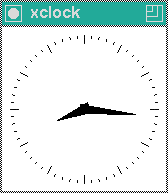
\includegraphics[width=\linewidth]{xclock.png}
		\end{minipage}
	\end{figure}
\end{frame}


\begin{frame}
	\frametitle{X11}
	\begin{itemize}
		\item Mrežni sustav
		\item Klijent (GUI aplikacija) se može nazaliti na udaljenom serveru
		\item X server ostvaruje vezu prema grafičkoj kartici
	\end{itemize}
	\begin{figure}
		\begin{minipage}{0.4\textwidth}
			\raggedleft
			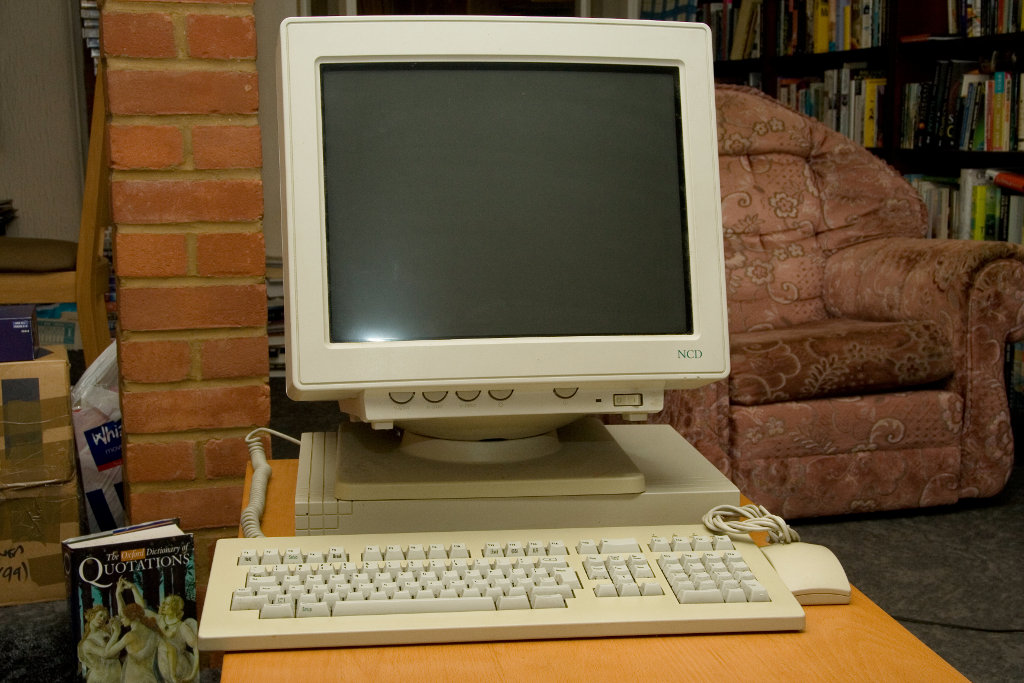
\includegraphics[width=\linewidth]{Xterminal.jpg}
			\caption*{NCD-88k X terminal}
		\end{minipage}
		\begin{minipage}{0.25\textwidth}
			\raggedright
			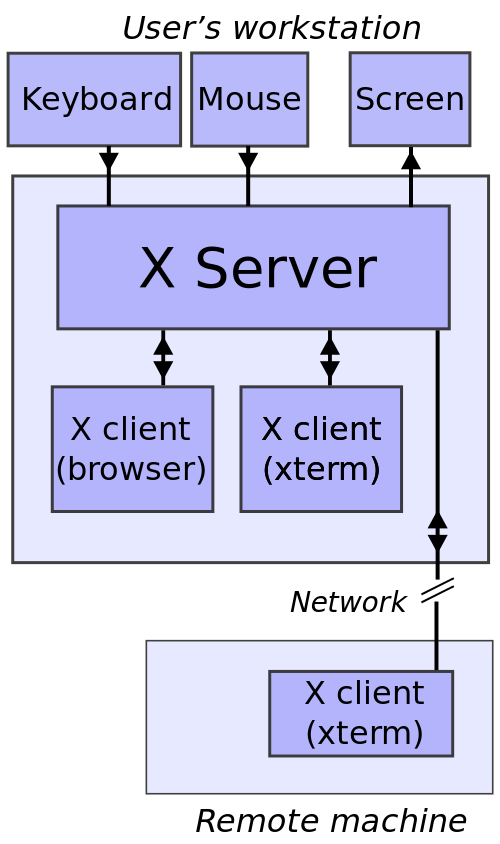
\includegraphics[width=\linewidth]{server_client.png}
		\end{minipage}
	\end{figure}
\end{frame}


\begin{frame}
	\frametitle{X11}
	\framesubtitle{Arhitektura}
	\centering
	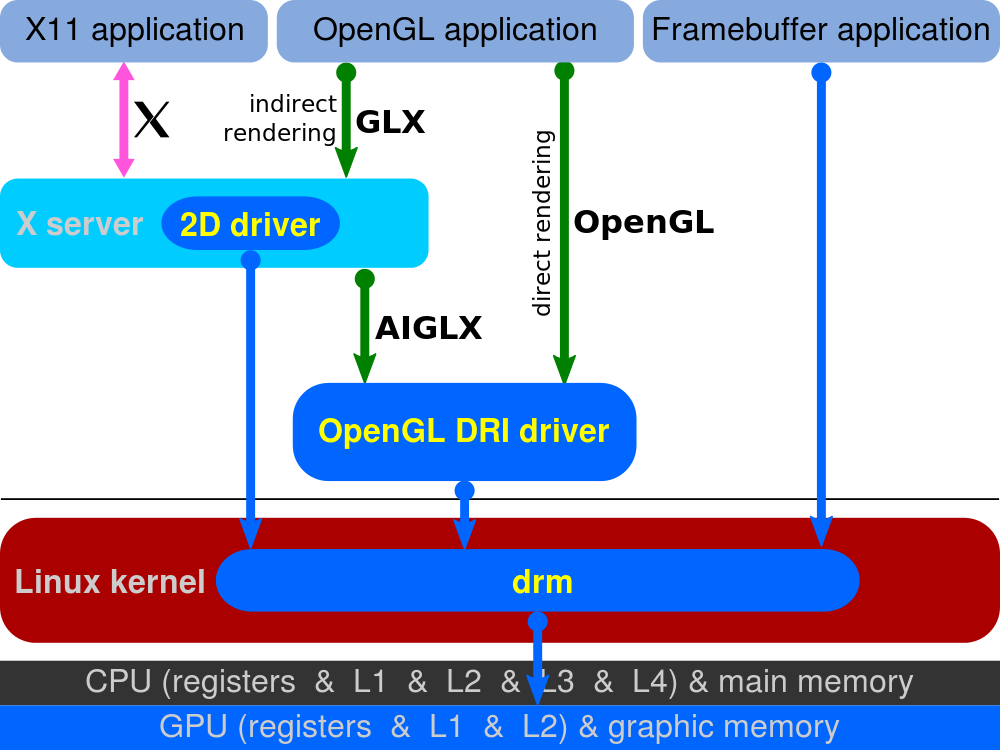
\includegraphics[width=0.75\textwidth]{graphics.png}
\end{frame}


\begin{frame}
	\frametitle{Window managers}
	\begin{itemize}
		\item Iscrtava i organizira prozore
		\item Stvara ukrase (naslovna traka, izbornici, scroll bar, \ldots)
		\item[]
		\item[] Primjeri
		\item[] Metacity, Xfwm, Kwin, Compiz, Mutter, Openbox, twm, \ldots
	\end{itemize}
\end{frame}


\begin{frame}
	\frametitle{GUI}
	Graphical shells
	\begin{itemize}
		\item Koriste window manager za prikaz cijelog GUI-a
		\item Omogućuje programa iz GUI-a, bolje upravljanje prozorima i radnim površinama, \ldots
	\end{itemize}
	Desktop environment
	\begin{itemize}
		\item Predstavlja kompletno rješenje grafičkog korisničkog sučelja
		\item U mnogim distribucijama dolazi neki predinstalirani desktop environment
		\item Mogu se po volji mijenjati; Ponovnom instalacijom ili odabirom između više instaliranih desktop environmenta pri loginu
	\end{itemize}
	
	Gnome, KDE, Xfce, Unity, MATE, Cinnamon, \ldots

\end{frame}


\begin{frame}
	\frametitle{Graphical shells}
	\framesubtitle{Gnome 3}
	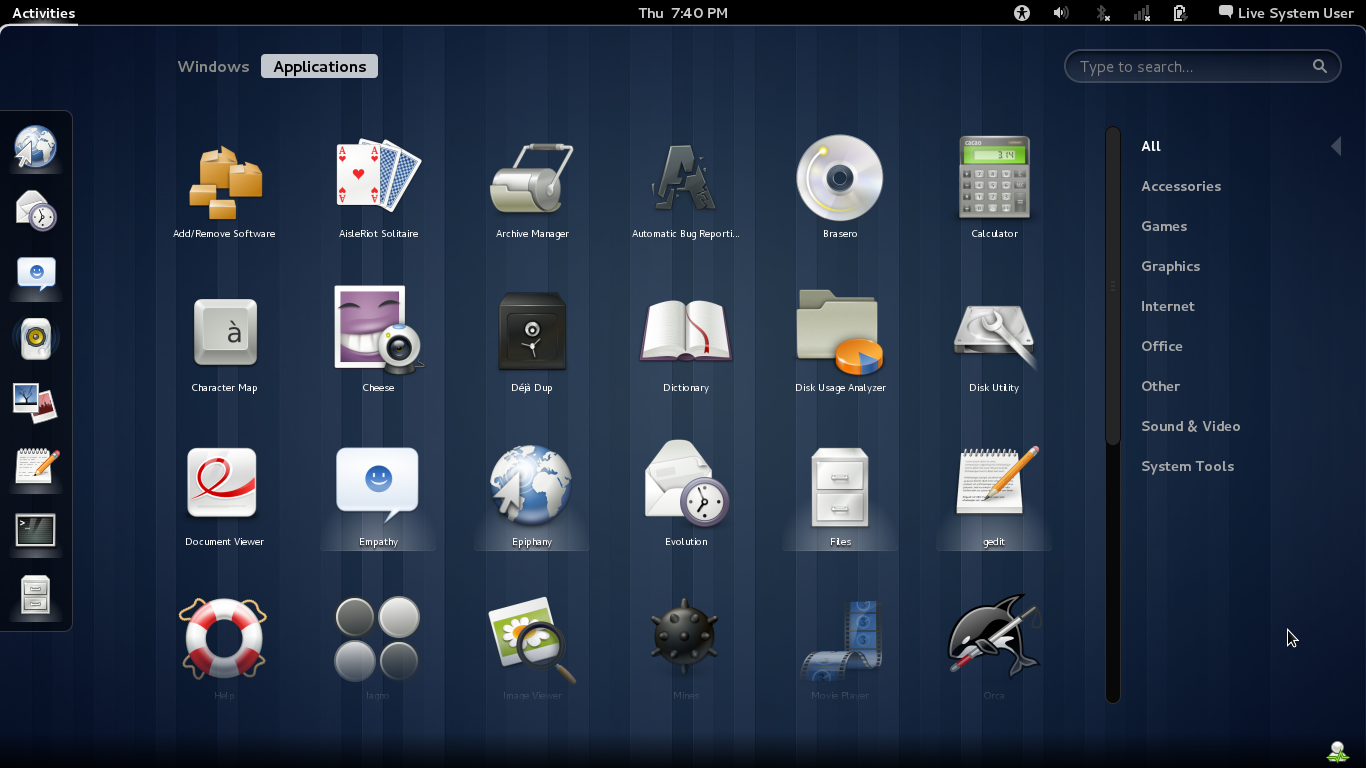
\includegraphics[width=\textwidth]{gnome3.png}
\end{frame}


\begin{frame}
	\frametitle{Graphical shells}
	\framesubtitle{Xfce}
	\centering
	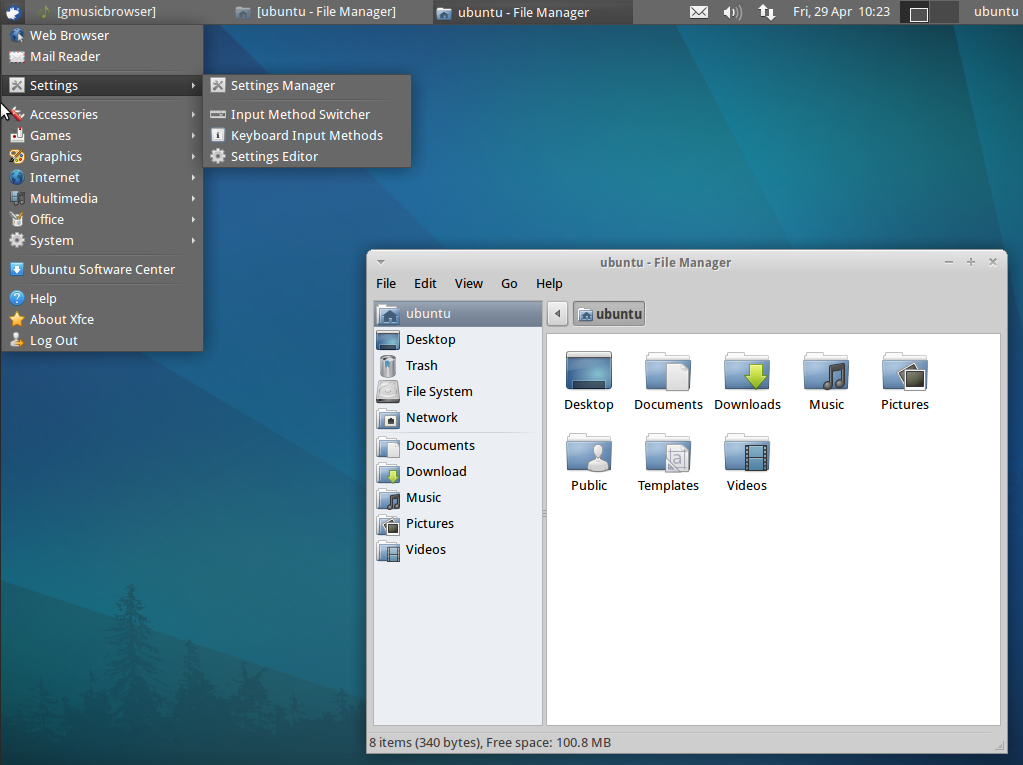
\includegraphics[width=0.75\textwidth]{xfce.png}
\end{frame}


\begin{frame}
	\frametitle{Graphical shells}
	\framesubtitle{KDE}
	\centering
	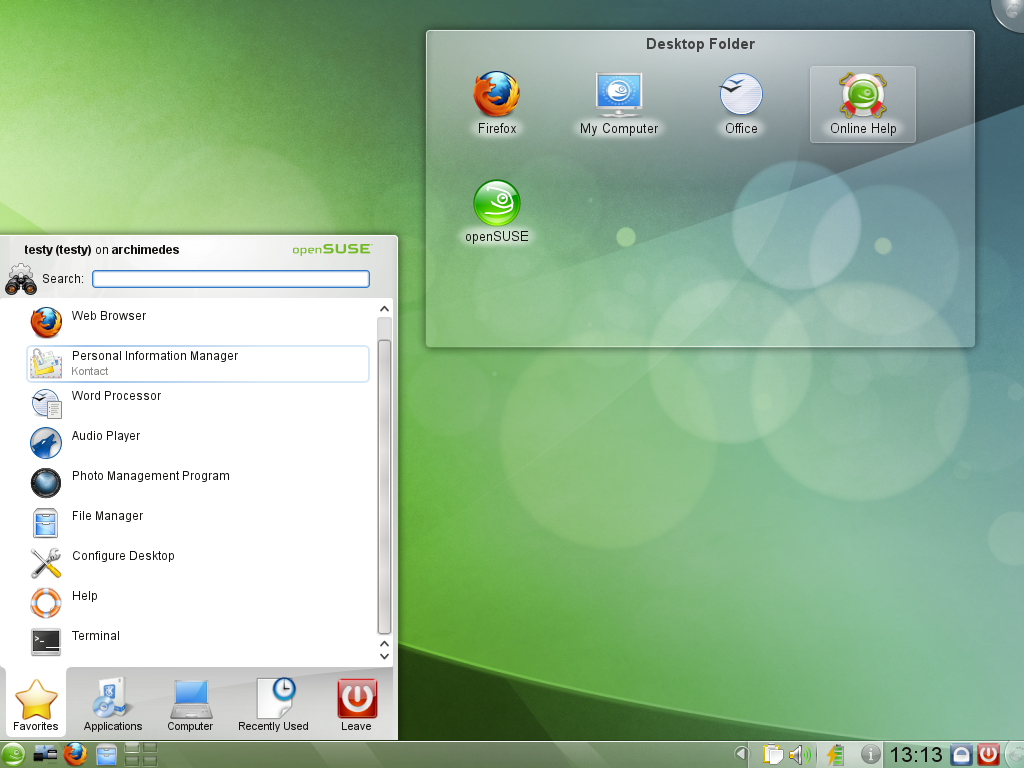
\includegraphics[width=0.75\textwidth]{kde.png}
\end{frame}


\begin{frame}
	\frametitle{Graphical shells}
	\framesubtitle{MATE}
	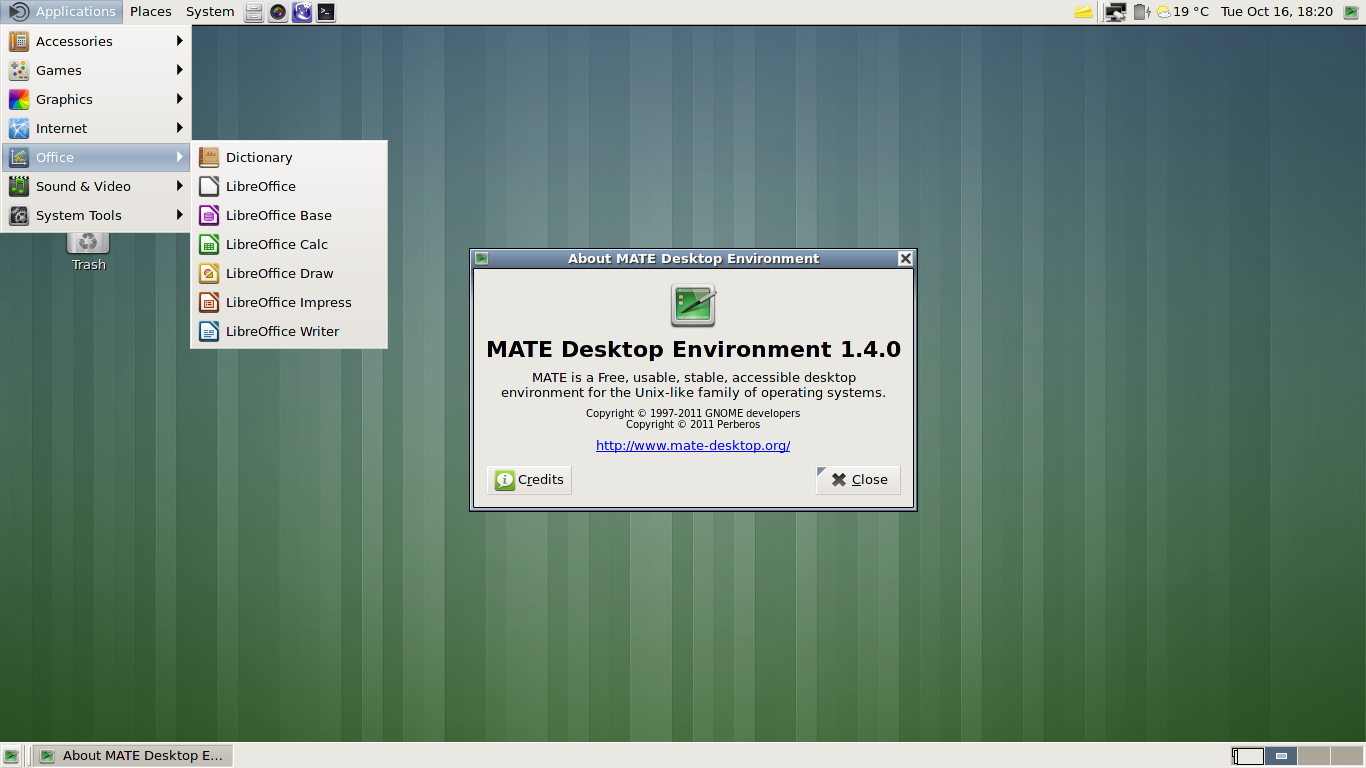
\includegraphics[width=\textwidth]{mate.png}
\end{frame}


\begin{frame}
	\frametitle{Display/Login Manager}
	\begin{itemize}
		\item Grafičko sučelje za logiranje
		\item Pokreće se kao servis - na startupu
		\item Redovito podržavaju različite konfiguracije sesije
		\item[] Na primjer izbor desktop environmenta koje želimo koristiti
	\end{itemize}
	\vfill
	Primjer
	\begin{itemize}
		\item GDM
		\item KDM
		\item LightDM
		\item Slim
		\item \ldots
	\end{itemize}
\end{frame}


\begin{frame}
	\frametitle{X11}
	\framesubtitle{Konfiguracija}
	\begin{itemize}
		\item Xorg konfiguracija
		\item[] \texttt{/etc/X11/}
		\begin{itemize}
			\item[] \texttt{/etc/X11/xorg.conf}
			\item[] \texttt{/etc/X11/xorg.conf.d}
		\end{itemize}
		\item[] \texttt{/etc/xorg.conf}
	\end{itemize}
	\vfill
	\texttt{Xorg :0 -configure}\\
	\texttt{startx} - Pokreće \texttt{\textbf{xinit}}
	\vfill
	\begin{itemize}
		{\ttfamily
			\item[] /etc/X11/xinit/xinitrc
			\item[] \textasciitilde/.xinitrc
		}
	\end{itemize}
\end{frame}


\begin{frame}
	\frametitle{Keyboard layout}
	\begin{itemize}
		\item \texttt{/etc/vconsole.conf}
		\begin{itemize}
			\item Postavke terminala
		\end{itemize}
		\item \texttt{loadkeys}
		\item X KeyBoard extension (xkb)
		\begin{itemize}
			\item[] \texttt{setxkbmap}
			\item[] Postavlja layout na X serveru
		\end{itemize}
		\item \texttt{localectl}
		\begin{itemize}
			\item Alat iz \texttt{systemd}
			\item Razne regionalne postavke, uključujući layout u terminalu i X serveru
		\end{itemize}
	\end{itemize}
\end{frame}



\section{Zvučni sustav}


\begin{frame}
	\frametitle{Arhitektura zvučnog sustava}
	\centering
	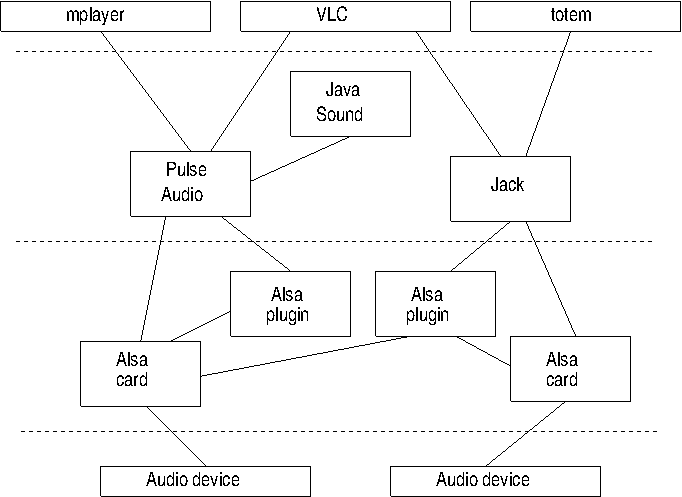
\includegraphics[width=0.8\textwidth]{sound_arch.png}
\end{frame}


\begin{frame}
	\frametitle{ALSA}
	Advanced Linux Sound Architecture (ALSA)\\
	\vfill
	\begin{itemize}
		\item Podrška zvučnog sustava uz hardversku razinu
		\item Pristup hardveru
		\item Hardverski mikseri
	\end{itemize}
	\vfill
\end{frame}


\begin{frame}
	\frametitle{ALSA}
	\framesubtitle{Naredbe, konfiguracija}
	\texttt{amixer}\\
	\texttt{alsamixer}\\
	\vfill
	\texttt{aplay}\\
	\texttt{arecord}\\
	\vfill
	Konfiguracijske datoteke
	\begin{itemize}
		\item[] \texttt{/etc/asound.conf}
		\item[] \texttt{\textasciitilde/.asoundrc}
	\end{itemize}
	\vfill
\end{frame}


\begin{frame}
	\frametitle{PulseAudio}
	\begin{itemize}
		\item Sound server
		\item Između aplikacije i ALSA
	\end{itemize}
	\vfill
	\begin{itemize}
		\item Omogućuje zvuk preko mreže
		\item Naprednije mixanje zvuka
	\end{itemize}
	\vfill
	\begin{itemize}
		\item[] \texttt{/etc/pulse}
		\item[] \texttt{\textasciitilde/.config/pulse}
		\begin{itemize}
			\item[] \texttt{daemon.conf}
			\item[] \texttt{default.pa}
		\end{itemize}
	\end{itemize}
\end{frame}


\begin{frame}
	\frametitle{Alternative}
	\textbf{Zvuk}\\
	Open sound system (OSS)
	\begin{itemize}
		\item Potisnuo ga ALSA
		\item Nakon verzije 4 opet često umjesto ALSA-e
	\end{itemize}
	\vspace{1em}
	JACK
	\begin{itemize}
		\item Sound server
		\item Profesionalni audio
	\end{itemize}
	\vfill
	\textbf{Grafika}\\
	Wayland
	\begin{itemize}
		\item Grafički server u razvoju
	\end{itemize}
	
\end{frame}


\begin{frame}
	\frametitle{Literatura}
	\url{https://wiki.archlinux.org/index.php/Xorg}\\
	\url{https://wiki.archlinux.org/index.php/Xinitrc}\\
	\url{https://wiki.archlinux.org/index.php/Start_X_at_login}
	\vfill
	\url{http://jan.newmarch.name/LinuxSound/Sampled/Architecture/}\\
	\url{http://www.alsa-project.org/main/index.php/Main_Page}\\
	\url{http://www.freedesktop.org/wiki/Software/PulseAudio/}
	\vfill
\end{frame}


\end{document}